   
								   
								   
												           Sejarah Garis Khatulistiwa Dan Prime Meridien
%Kelompok 4
% Eka Pratama Putra (1154023)
% Deni Braja Astrajingga (1154066)
% Luqman Nurfajri (1154054)
% Shinta Amelia (1154047)
% Yoshi Ricowandi Nababan (1154125)

														   
\section {Pendahuluan}

\subsection{pengertian garis khatulistiwa}	

	Dalam sebuah artikel dari Muhammad Adieb yang menyebutkan bahwa garis khatulistiwa merupakan garis lintang dari 0 derajat sampai dengan 90 derajat 
di kutub bumi. Jadi, nilai lintang berkisar antara 0° sampai dengan 90°. Di sebelah selatan garis khatulistiwa disebut lintang selatan (LS) dengan 
tanda negatif (-) dan di sebelah utara garis khatulistiwa disebut lintang utara (LU) yang diberi tanda positif (+). \cite {adieb2014studi}.

\subsection{pengertian prime meridian}
	
	Dalam sebuah artikel dari Mohd Zuhdi yang menyebutkan bahwa Prime meridian atau meridian Greenwich adalah nilai koordinat garis bujur dimulai dari 
bujur 0 derajat yaitu di Greenwich, kemudian membesar ke arah timur dan barat sampai bertemu kembali di Garis batas internasional yaitu terletak 
di Selat Bering dengan nilai 180 derajat. \cite {zuhdi2012sistem}.

	Dalam sebuah artikel lain oleh Andi Sunyoto yang menyebutkan bahwa Prime meridian adalah sebuah garis virtual yang melewati sebuah kota 
bernama Greenwich di Inggris. \cite{sunyoto2009api}.

\section {Isi}

\subsection{sistem koordinat bumi}
	
	Menurut sebuah artikel dari Mohd Zuhdi yang menyebutkan bahwa dalam sebuah artikel dari Mohd Zuhdi yang menyebutkan bahwa sistem koordinat dimaksudkan 
untuk memberikan pengalamatan terhadap setiap lokasi di permukaan bumi. pengalamatan dengan sistem koordinat didasarkan atas jarak timur sampai dengan barat 
dan utara sampai dengan selatan suatu tempat dari suatu titik pangkal tertentu. jarak diukur dalam satuan derajat dengan sudut yang dibentuk dari titik 
pangkal ditetapkan yang berada di perpotongan belahan utara sampai dengan selatan bumi (garis khatulistiwa) dengan garis yang membelah bumi bagian timur sampai 
dengan barat melewati kota GreenWhich di Inggris.

	
\begin{figure}[ht]
\centerline{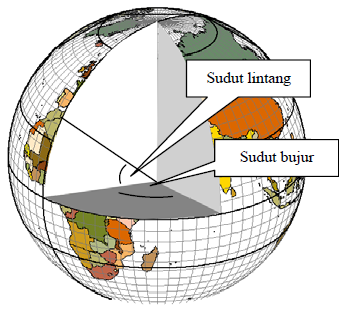
\includegraphics[width=1\textwidth]{figures/garis_lintang_dan_bujur.PNG}}
\caption{menjelaskan tentang sudut lintang dan bujur pada bumi.}
\label{garis_lintang_dan_bujur}
\end{figure}

Pada gambar \ref{garis_lintang_dan_bujur} menjelaskan tentang sudut lintang dan bujur pada bumi.

	Posisi suatu tempat di alamatkan dengan nilai koordinat garis bujur (longitude) dan lintang (latitude) yang melalui tempat itu. Garis bujur (longitude), 
biasanya juga disebut garis meridian, yaitu merupakan garis lurus yang menyambungkan dari kutub utara sampai selatan bumi. Nilai koordinat garis bujur ini dimulai dari
bujur 0 derajat yaitu di Greenwich, kemudian membesar ke arah timur dan barat sampai bertemu kembali di Garis batas internasional yaitu terletak 
di Selat Bering dengan nilai 180 derajat. Garis bujur 0 derajat sering disebut prime meridien atau meridian Greenwich. Garis bujur ke arah barat diberi 
nilai negatif dan disebut bujur barat (west longitude) serta disingkat BB. Sedangkan garis bujur yang ke arah timur diberi nilai positif 
dan disebut bujur timur (east longitude) disingkat BT. Nilai koordinatnya didasarkan atas besarnya sudut yang terbentuk dari bujur 0 ke garis bujur tersebut
 melalui pusat bumi.

	Adapun nilai koordinat lintang dimulai dari garis lingkaran khatulistiwa yang diberi nilai 0 derajat. Selanjutnya garis-garis lintang yang lain berupa 
lingkaran-lingkaran paralel (sejajar) khatulistiwa berada di sebelah utara dan selatan khatulistiwa. Lingkaran paralel di selatan disebut garis lintang selatan (LS)
dan diberi nilai negatif, sedangkan lingkaran paralel di utara  diberi  nilai positif dan disebut garis lintang utara (LU). Nilai maksimum koordinat 
garis lintang adalah 90 derajat yaitu terletak di kutub-kutub bumi.

	Lingkaran paralel yang merupakan representasi garis lintang ini semakin mengecil ukurannya dengan semakin jauh dari khatulistiwa. Sehingga jarak 1 derajat 
timur sampai barat hanya beberapa meter saja. Itu sebabnya grid yang dibuat dari garis lintang dan garis bujur, tampaak berupa bujur sangkar di khaatulistiwa 
dan berubah menjadi persegi panjang di daerah dekat kutub. \cite {zuhdi2012sistem}.

\subsection (pemanfaatan prime meridian)

	Meridian Utama atau Prime Meridien digunakan untuk menentukan waktu di dunia, metode penentuannya akan dijelaskan sebagai berikut

\subsubsection(sistem penentuan waktu dunia)
	
	Menurut sebuah artikel dari Misbah Khusurur dan Jaenal Arifin yang menyebutkan bahwa Waktu Universal (bahasa Inggris Universal Time, disingkat UT)
adalah satu ukuran waktu yang didasari oleh rotasi bumi. Satuan ini adalah model perhitungan modern dari GMT (Greenwich Mean Time), yaitu mean waktu matahari 
di meridian di Greenwich, Inggris, yang biasanya dianggap sebagai bujur geografis 0 derajat GMT ini merupakan waktu 4 pertengahan yang yang di dasari oleh 
garis bujur yang melalui Greenwhich (BB/BT 0°) dan digunakan sebagai standar waktu Dunia Internasional.
	
	Sebelum diperkenalkannya standar waktu, setiap kota menyetel waktunya sesuai dengan posisi matahari di tempat masing-masing. Sistem ini bekerja 
dengan baik sampai diperkenalkannya transportasi kereta api untuk berpergian dengan cepat. akan tetapi, memerlukan seseorang untuk terus-menerus mencocokan 
jamnya dengan waktu lokal yang berbeda-beda dari satu kota ke kota lain. Standar waktu, dimana semua jam di dalam satu daerah menggunakan waktu yang sama, 
dibuat untuk memecahkan masalah perbedaan waktu seperti dalam perjalanan kereta api di atas.

	Standar waktu ini membagi bumi kedalam beberapa bagian ”zona waktu”, masing-masing bagiannya mencakupi dengan paling sedikit 15 derajat. Semua jam di dalam
zona waktu ini disetel sama dengan jam lainnya, tapi berbeda sebanyak satu jam dari jam-jam di zona waktu yang bertetanggaan. 
Waktu lokal di Royal Greenwich Observatory di Greenwich, Inggris, dipilih sebagai standard waktu dunia setelah terjadi 
Konferensi Meridian Internasional tahun 1884, yang memicu penyebaran pemakaian Greenwich Mean Time untuk menyetel jam di dalam suatu daerah. 
Lokasi ini dipilih sampai tahun 1884, 66 % dari semua peta dan tabel menggunakan greenwhich sebagai meridian utama (prime meridian).

\begin{figure}[ht]
\centerline{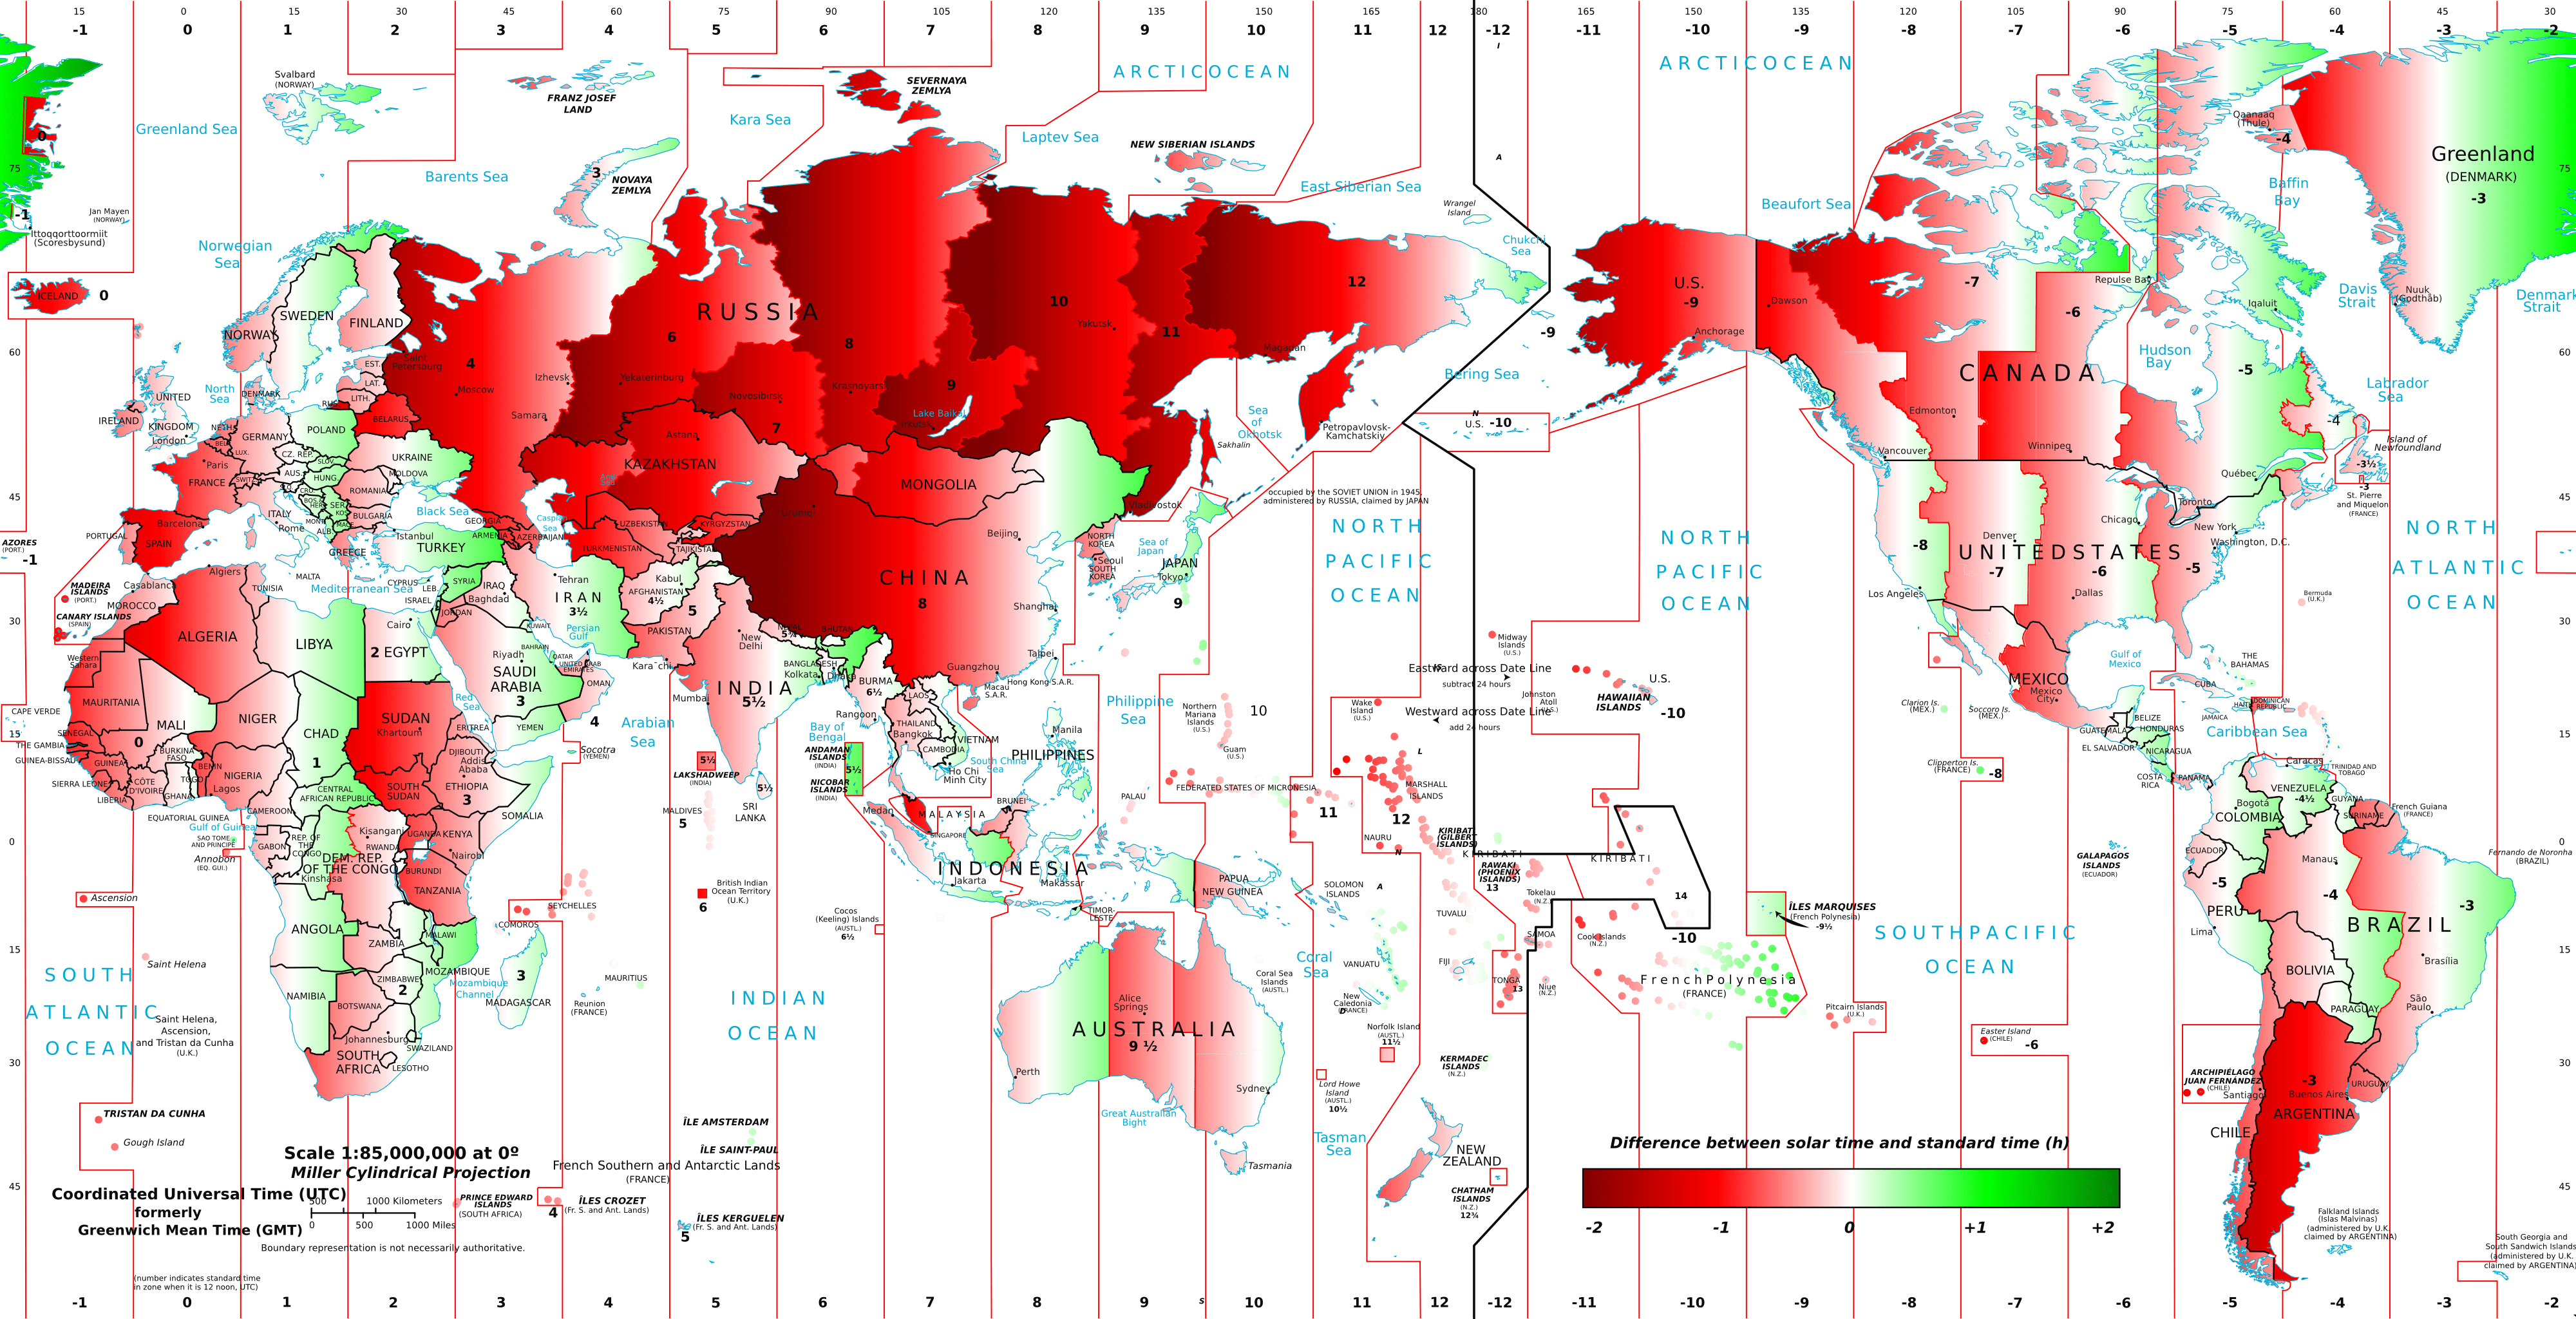
\includegraphics[width=1\textwidth]{figures/pembagian_waktu_dunia.PNG}}
\caption{menjelaskan tentang zona waktu pada tiap belahan dunia.}
\label{pembagian_waktu_dunia}
\end{figure}

Pada gambar \ref{pembagian_waktu_dunia} menjelaskan tentang zona waktu pada tiap belahan dunia.

	Perbedaan GMT dengan waktu pertengahan setempat di luar Greenwich adalah tergantung besar kecilnya Garis Bujur (BB/BT) dan dapat dirumuskan 
sebagai berikut:
\begin{equation}
WP x = GMT + BT, 
\end {equation}
atau 
\begin{equation}
WP x = GMT – BB
\end {equation}

\begin{equation}
GMT = WP x - BT, 
atau
\end{equation}
\begin{equation}
GMT = WP x + BB
\end{equation}
Contohnya sebagai berikut:

\begin {enumerate}
\item
Diketahui BT Semarang = 110° 26’
Pada saat GMT menunjukkan pukul 11.30, 
\begin{equation}
WP x = WP Semarang = 11.30 + 110° 26’
= 11.30 + 7 j 21m 44dt
= 18 j 51 m 44 dt
\end{equation}

\item
Diketahui BT Semarang = 100° 26’
Pada saat WP Semarang menunjukkan pukul 19.54,
\begin{equation}
GMT = 19.54 - 100° 26’
    = 19.54 - 8 j 24m 0dt
    = 11.30
\end{equation}
\end {enumerate}

\cite {khusurur2016mengenal}

\subsection {Dampak wilayah yang dilalui oleh garis khatulistiwa}

	Menurut sebuah artikel dari Yanti, Ari Hepi and Dhewiyanty, Varla and Setyawati, Tri Rima yang menyebutkan bahwa daerah yang dilalui garis khatulistiwa 
memiliki iklim tropis dengan suhu udara cukup tinggi dan kelembaban yang tinggi. Contoh daerah yang dilalui garis khatulistiwa yaitu Kalimantan Barat
suhu udara di Kalimantan Barat pada tahun 2013 berkisar antara 21,5oC-34,3oC (BPS Kalbar, 2014). \cite {yanti2015prevalensi}

	Masih ada lagi beberapa negara yang dilalui oleh garis khatulistiwa yang terdapat pada gambar \ref{tabel_negara_yang_dilalui_garis_khatulistiwa}

\begin{figure}[ht]
\centerline{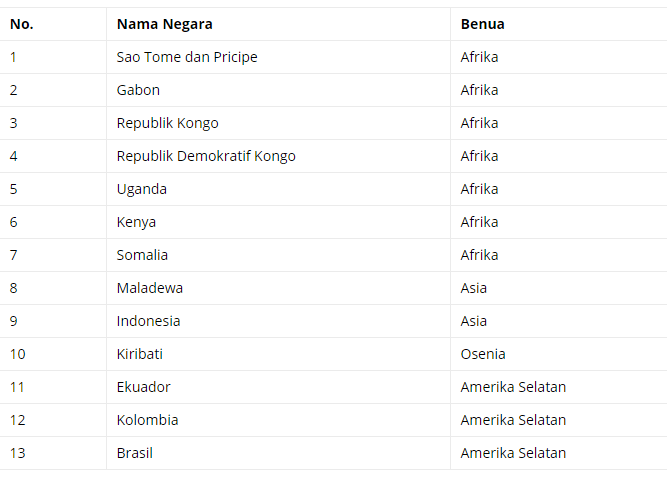
\includegraphics[width=1\textwidth]{figures/tabel_negara_yang_dilalui_garis_khatulistiwa.PNG}}
\caption{list negara yang dilalui garis khatulistiwa.}
\label{tabel_negara_yang_dilalui_garis_khatulistiwa}
\end{figure}

	Pada gambar \ref{tabel_negara_yang_dilalui_garis_khatulistiwa} disebutkan negara - negara yang dilalui oleh garis khatulistiwa yaitu Sao Tome dan Pricipe 
yang terdapat pada benua Afrika, Gabon yang terdapat di benua Afrika, Republik Kongo yang terdapat di benua Afrika, Republik Demokratif Kongo yang terdapat 
di benua Afrika, Uganda yang terdapat di benua Afrika, Kenya yang terdapat di benua Afrika, Somalia yang terdapat di benua Afrika, Maladewa yang terdapat 
di benua Asia, Indonesia yang terdapat di benua Asia, Negara Kiribati , Ekuador yang terdapat di benua Amerika Selatan, Kolombia 
yang terdapat di benua Amerika Selatan, dan Brasil yang terdapat di benua Amerika Selatan
	
	untuk lebih detailnya terdapat pada gambar \ref{Peta_Dunia_Negara_Khatulistiwa}
	
\begin{figure}[ht]
\centerline{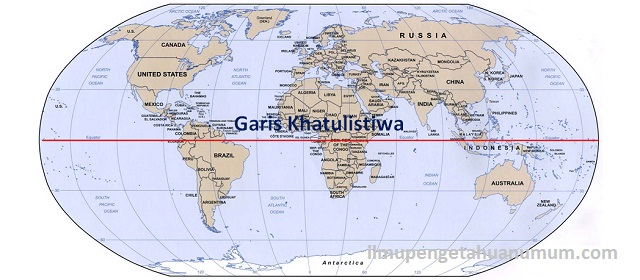
\includegraphics[width=1\textwidth]{figures/Peta_Dunia_Negara_Khatulistiwa.JPG}}
\caption{wilayah di dunia yang dilewati garis khatulistiwa.}
\label{Peta_Dunia_Negara_Khatulistiwa}
\end{figure}

\subsubsection {Peristiwa Equinox}

	Dalam sebuah artikel dari Mutoha Arkanudin yang menyebutkan bahwa selama setahun Matahari berubah posisi dari Utara ke Selatan dan sebaliknya. 
Posisi tersebut sering disebut sebagai Gerak Musim Matahari. Equinox adalah saat dimana posisi matahari berada tepat di Ekuator atau garis katulistiwa. 
Ini adalah bagian dari siklus tahunan pergerakan harian semu matahari saat terbit, melintas dan terbenam yang disebabkan oleh kemiringan sumbu bumi
terhadap bidang orbitnya yaitu sebesar 66.56 derajat. Selama setahun terjadi dua kali Equinox yaitu Maret Equinox yang terjadi setiap tanggal 21 Maret dan September
Ekuinox yang terjadi setiap tanggal 23 September. 

	Saat terjadi peristiwa Equinox posisi Matahari terbenam akan tepat berada di titik Barat sehingga dengan menambah sudut kemiringan arah kiblat 
terhadap titik Barat maka arah kiblat yang sesungguhnya kan kita dapatkan. 

	Selain Equinox matahari juga akan berada di titik paling Utara pada 21 Juni dan berada di titik paling Selatan pada 22 Desember yang dikenal dengan 
istilah Solstice. Pada saat Juni Solstice, Matahari akan terbenam tepat di sudut serong terhadap arah Barat sebesar 23,5 derajat ke arah Utara
sehingga untuk menuju ke arah kiblat yang tepat dapat tinggal menambahkan kekurangan penyerongan angka arah kiblat yang didapatkan dari hasil perhitungan 
menggunakan rumus segitiga bola. Sedangakan pada saat Desember Solstice matahari terbenam di Selatan titik Baratsebesar 23,5 derajat.\cite {arkanudin2008teknik}.

\section {Penutup}

\subsection{Kesimpulan}
	
	Garis khatulistiwa merupakan garis lintang dari 0 derajat sampai dengan 90 derajat di kutub bumi. Prime meridian atau meridian Greenwich adalah 
nilai koordinat garis bujur dimulai dari bujur 0 derajat yaitu di Greenwich, kemudian membesar ke arah timur dan barat sampai bertemu kembali di Garis batas 
internasional yaitu terletak di Selat Bering dengan nilai 180 derajat. Sistem koordinat dimaksudkan untuk memberikan pengalamatan terhadap setiap lokasi 
di permukaan bumi. Meridian Utama atau Prime Meridien digunakan untuk menentukan waktu di dunia, metode penentuan mengikuti Waktu Universal (bahasa 
Inggris Universal Time, disingkat UT) adalah satu ukuran waktu yang didasari oleh rotasi bumi. daerah yang dilalui garis khatulistiwa memiliki iklim tropis 
dengan suhu udara cukup tinggi dan kelembaban yang tinggi.

\subsection{Saran}

	Dalam artikel ini belum ada penjelasan mengenai sejarah garis khatulistiwa dan prime meridien, maka diharapkan untuk  kedepannya dilengkapi dengan 
informasi mengenai sejarah dari garis khatulistiwa dan prime meridien.	